\documentclass[12pt]{article}

\usepackage[english]{babel}
\usepackage[utf8x]{inputenc}
\usepackage[T1]{fontenc}
\usepackage{parskip}
\usepackage{lipsum}
\usepackage[a4paper, total={6in, 8in}]{geometry}
\usepackage{setspace}
\usepackage[superscript]{cite}
\usepackage{xcolor}
\usepackage{hyperref}
\usepackage{enumitem}
\usepackage{listings}
\usepackage{amsmath}
\usepackage{amssymb}
\usepackage{ifsym}
\usepackage{amssymb}
\usepackage{tikz}

\definecolor{azzurro}{cmyk}{1,0.33,0,0.13}
\definecolor{arancione}{cmyk}{0,0.41,1,0}
\definecolor{verde}{cmyk}{0.44,0,0.38,0.31}
\definecolor{viola}{rgb}{0.58,0,0.82}
\definecolor{bianco}{rgb}{0.95, 0.95, 0.92}
% C style
\lstdefinestyle{CStyle}{
    backgroundcolor=\color{bianco},   
    commentstyle=\color{verde},
    keywordstyle=\color{viola},
    numberstyle=\tiny\color{arancione},
    stringstyle=\color{azzurro},
    basicstyle=\footnotesize,
    breakatwhitespace=false,         
    breaklines=true,                 
    captionpos=b,                    
    keepspaces=true,                 
    numbers=left,                    
    numbersep=5pt,                  
    showspaces=false,                
    showstringspaces=false,
    showtabs=false,                  
    tabsize=2,
    language=C
}
\lstset{
  basicstyle=\ttfamily,
  columns=fullflexible,
  frame=single,
  breaklines=true,
  postbreak=\mbox{\textcolor{red}{\(\hookrightarrow\)}\space},
}


% change margins within the geometry package and eventually the font size

\begin{document}
	
\begin{flushright}
	\today
\end{flushright}
{\Large \textbf{Assignment 4}}
	
{\large Query Optimization}
	
\textsc{Ilaria Battiston - 03723403} \\
\textsc{Mareva Zenelaj - 03736071}
	
\rule{\linewidth}{0.5pt}

\section{First exercise}
\subsection{Query Graph}
This query graph assumes four relations $R_1$, $R_2$, $R_3$, $R_4$, each of them with cardinality 10. We are considering the following query graph:

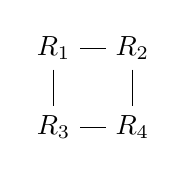
\begin{tikzpicture}
  \node (R0) at (0,0) {$R_1$};
  \node (R1) [right of=R0] {$R_2$};
  \node (R2) [below of=R0] {$R_3$};
  \node (R3) [right of=R2] {$R_4$};
  \draw (R0) -- (R1);
  \draw (R0) -- (R2);
  \draw (R1) -- (R3);
  \draw (R2) -- (R3);
\end{tikzpicture}

The selectivities of the query graph are:
\begin{itemize}
	\item $R_1 \bowtie R_2 = 0.4$;
	\item $R_1 \bowtie R_3 = 0.5$;
	\item $R_2 \bowtie R_4 = 0.49$;
	\item $R_3 \bowtie R_4 = 0.6$.
\end{itemize}

The algorithm GreedyOperatorOrdering will perform the following steps:
\begin{enumerate}
	\item Join $R_1$ and $R_2$;
	\item Join $R_3$ and $R_4$;
	\item Join the two results.
\end{enumerate}
$$ C_{out}((R_1 \bowtie R_2) \bowtie (R_3 \bowtie R_4)) = 40 + 60 + 588 = 688$$

However, there exists another join ordering giving a better result:
$$ C_{out}((R_1 \bowtie R_3) \bowtie (R_2 \bowtie R_4)) = 50 + 49 + 588 = 687$$

\subsection{Join Tree}
Execution of GreedyOperatorOrdering:
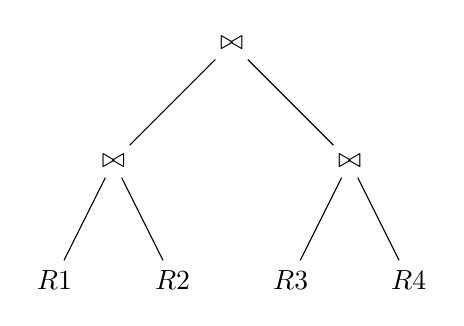
\begin{tikzpicture}[sibling distance=3cm, level 2/.style={sibling distance=1.5cm}]
  \node (j1) {$\bowtie$} {
    child {
      node (j2) {$\bowtie$}
      child {
        node (j3) {$R1$}
      }
      child {
        node (j6) {$R2$}
      }
    }
    child {
      node (j7) {$\bowtie$}
      child {
      	node (j8) {$R3$}
      }
      child {
      	node (j8) {$R4$}
      }
    }
  };
\end{tikzpicture}

Optimal join tree:
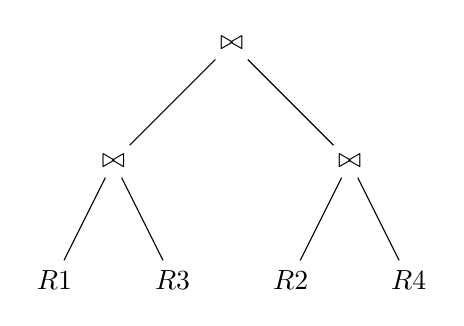
\begin{tikzpicture}[sibling distance=3cm, level 2/.style={sibling distance=1.5cm}]
\node (j1) {$\bowtie$} {
	child {
		node (j2) {$\bowtie$}
		child {
			node (j3) {$R1$}
		}
		child {
			node (j6) {$R3$}
		}
	}
	child {
		node (j7) {$\bowtie$}
		child {
			node (j8) {$R2$}
		}
		child {
			node (j8) {$R4$}
		}
	}
};
\end{tikzpicture}

\subsection{GreedyJoinOrdering-1}
In this example the proposed weight function corresponds to the cardinality. However, all relations have the same cardinality, therefore it is assumed that the chosen ordering is the natural one:

\begin{tikzpicture}[sibling distance=2.5cm]
\node (j1) {$\bowtie$} {
	child {
		node (j2) {$\bowtie$} 
		child {
			node (j3) {$\bowtie$}
			child {
				node (j5) {$R_1$}
			}
			child {
				node (j6) {$R_2$}
			}
		}
		child {
			node (j6) {$R_3$}
		}
	}
	child {
		node (j7) {$R_4$}
	}
};
\end{tikzpicture}

$$C_{out}(((R_1 \bowtie R_2) \bowtie R_3) \bowtie R_4) = 40 + 200 + 588 = 828$$

\newpage
\subsection{GreedyJoinOrdering-2}
The algorithm joins according to selectivity:

\begin{tikzpicture}[sibling distance=2.5cm]
\node (j1) {$\bowtie$} {
	child {
		node (j2) {$\bowtie$} 
		child {
			node (j3) {$\bowtie$}
			child {
				node (j5) {$R_1$}
			}
			child {
				node (j6) {$R_2$}
			}
		}
		child {
			node (j6) {$R_4$}
		}
	}
	child {
		node (j7) {$R_3$}
	}
};
\end{tikzpicture}

$$ C_{out}(((R_1 \bowtie R_2) \bowtie R_4) \bowtie R_3) = 40 + 196 + 588 = 824$$

\subsection{GreedyJoinOrdering-3}
In this example we only show the optimal join tree with all the possible $C_{out}$ combinations:
\begin{itemize}
	\item Starting from $R_1$: $ C_{out}(((R_1 \bowtie R_2) \bowtie R_4) \bowtie R_3) = 40 + 196 + 588 = 824$;
	\item Starting from $R_2$: $ C_{out}(((R_2 \bowtie R_2) \bowtie R_4) \bowtie R_3) = 40 + 196 + 588 = 824$;
	\item Starting from $R_3$: $ C_{out}(((R_3 \bowtie R_1) \bowtie R_2) \bowtie R_4) = 50 + 200 + 588 = 838$;
	\item Starting from $R_4$: $ C_{out}(((R_4 \bowtie R_2) \bowtie R_1) \bowtie R_3) = 49 + 196 + 588 = 833$.
\end{itemize}

Clearly, the minimum value is achieved starting from $R_1$ or $R_2$, hence the optimal tree is:

\begin{tikzpicture}[sibling distance=2.5cm]
\node (j1) {$\bowtie$} {
	child {
		node (j2) {$\bowtie$} 
		child {
			node (j3) {$\bowtie$}
			child {
				node (j5) {$R_1$}
			}
			child {
				node (j6) {$R_2$}
			}
		}
		child {
			node (j6) {$R_4$}
		}
	}
	child {
		node (j7) {$R_3$}
	}
};
\end{tikzpicture}




\end{document}